% Section 4: Results
All values below are audit-sourced (Step-1 independent audit, PASS).
Seeds are reported per-draw; means/SDs are over the three fresh seeds.

\paragraph{Benchmark gain (\dA{}) and correct-image dependence (\dG{}).}
\begin{table}[t]
\centering
\small
\begin{tabular}{lcccc}
\toprule
family & checkpoint & \dA{} & $G$ & \dG{} \\
\midrule
\qwen{} & seed-0 & $+0.0542$ & $0.3522$ & $+0.0456$ \\
\qwen{} & seedA & $+0.0547$ & $0.3544$ & $+0.0478$ \\
\qwen{} & seedB & $+0.0456$ & $0.3444$ & $+0.0378$ \\
\qwen{} & seedC & $+0.0515$ & $0.3531$ & $+0.0465$ \\
\smol{} & seed-0 & $+0.0287$ & $0.2975$ & $+0.0305$ \\
\smol{} & seedA & $+0.0305$ & $0.3007$ & $+0.0337$ \\
\smol{} & seedB & $+0.0323$ & $0.2957$ & $+0.0287$ \\
\smol{} & seedC & $+0.0319$ & $0.2993$ & $+0.0323$ \\
\qwennew{} & tuned & $+0.0323$ & $0.3827$ & $+0.0355$ \\
\bottomrule
\end{tabular}
\caption{Headline adaptation quantities. $G = A_{\text{normal}} -
A_{\text{shuffle}}$; \dG{} is relative to zero-shot. All values from the
independent audit.}
\label{tab:headline}
\end{table}

\Cref{tab:headline} reports the per-seed quantities. \dA{} is positive for
every seed on both backbones (7B fresh-seed mean $+0.0506 \pm 0.0046$; 2B
fresh-seed mean $+0.0316 \pm 0.0009$). The normal-minus-shuffle gap $G$
widens under tuning in every family, and the zero-shot-relative change
\dG{} is positive for every seed (7B fresh-seed mean $+0.0440 \pm 0.0054$;
2B fresh-seed mean $+0.0316 \pm 0.0026$). Shuffle accuracy itself stays
flat (e.g., 2B zero-shot 0.4692 vs.\ tuned 0.4674--0.4729), so the gain is
in using the correct image, not in memorizing image-independent answers.

\begin{figure}[t]
\centering
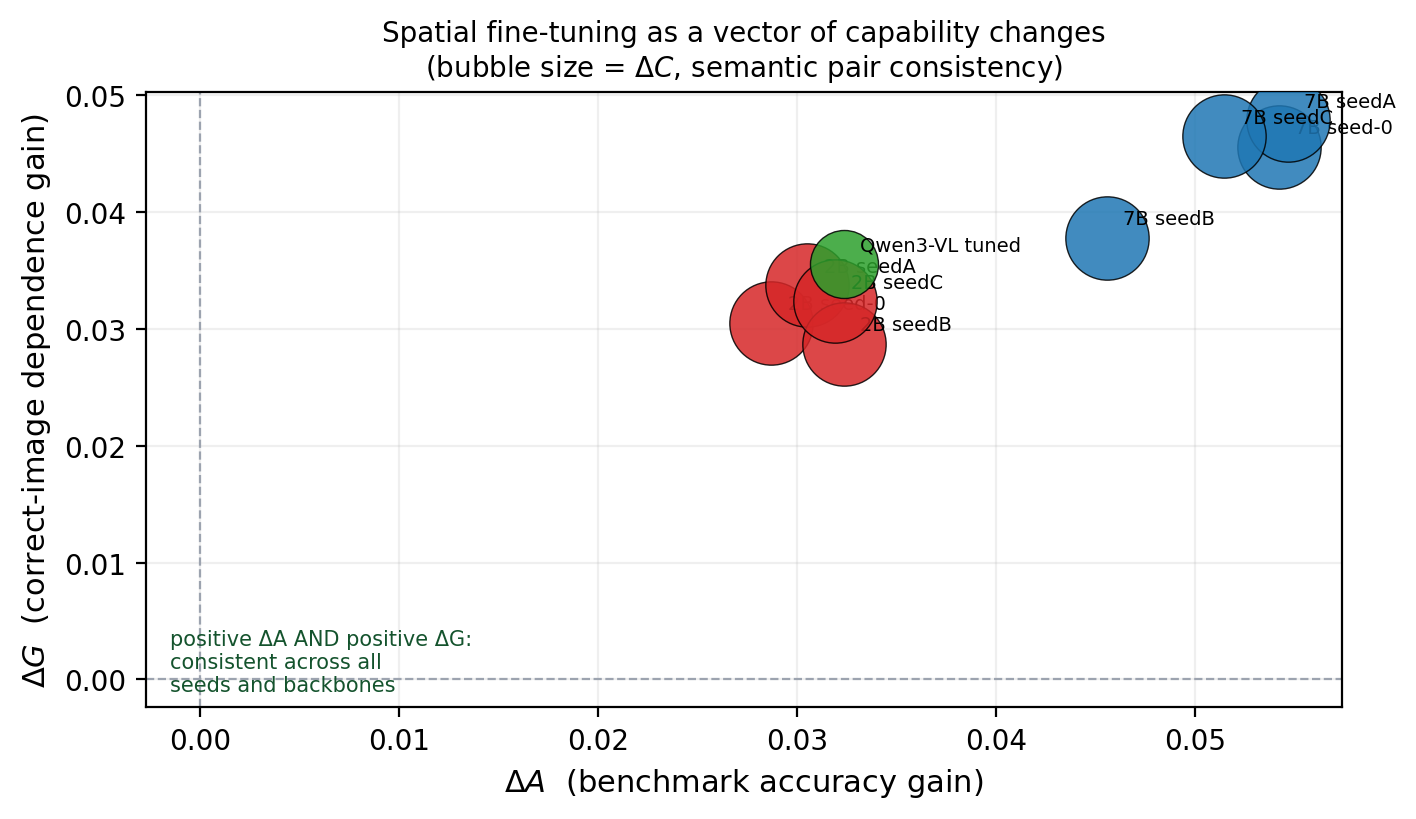
\includegraphics[width=\columnwidth]{fig/fig1_conceptual.png}
\caption{Conceptual decomposition: \dA{} (x) versus \dG{} (y) for all nine
checkpoints (7B seed-0 + three seeds, 2B seed-0 + three seeds, \qwennew{}
tuned); bubble size encodes \dC{} (semantic pair consistency change).
All points lie in the positive-positive quadrant.}
\label{fig:conceptual}
\end{figure}

\paragraph{Semantic pair consistency (\dC{}, relcomp).}
\begin{table}[t]
\centering
\small
\begin{tabular}{lcc}
\toprule
family & checkpoint & $C_{\text{pair}}$ (relcomp) \\
\midrule
\qwen{} & seed-0 & $0.6772$ \\
\qwen{} & seedA & $0.6637$ \\
\qwen{} & seedB & $0.6547$ \\
\qwen{} & seedC & $0.6652$ \\
\smol{} & seed-0 & $0.5015$ \\
\smol{} & seedA & $0.4985$ \\
\smol{} & seedB & $0.5045$ \\
\smol{} & seedC & $0.5105$ \\
\bottomrule
\end{tabular}
\caption{Relcomp pair consistency ($n=666$). Fresh seeds stay within 0.05
of the legacy General checkpoint in both families.}
\label{tab:relcomp}
\end{table}

\Cref{tab:relcomp} shows relcomp $C_{\text{pair}}$. Fresh seeds cluster
tightly around seed-0 in both families (7B: 0.6547--0.6652 vs.\ 0.6772; 2B:
0.4985--0.5105 vs.\ 0.5015); the audit confirms every fresh seed is within
0.05 of the legacy General checkpoint. The facing-antonym diagnostic
(facingcomp, $n=103$) shows the same pattern of tight seed clustering
(2B seed-0 0.3469; fresh seeds 0.3429--0.3714).

\paragraph{Transformation behavior under global reflection (Tier C).}
\begin{table}[t]
\centering
\small
\begin{tabular}{llccc}
\toprule
family & checkpoint & $A_{\text{transform}}$ & $C_{\text{pair}}$ & both\_correct \\
\midrule
\qwen{} & zero-shot & 0.6367 & 0.6163 & 0.5388 \\
\qwen{} & seed-0 & 0.6571 & 0.6857 & 0.5959 \\
\qwen{} & seedA & 0.6490 & 0.6490 & 0.5796 \\
\qwen{} & seedB & 0.6571 & 0.6898 & 0.6041 \\
\qwen{} & seedC & 0.6449 & 0.6653 & 0.5837 \\
\smol{} & zero-shot & 0.4980 & 0.3184 & 0.2531 \\
\smol{} & seed-0 & 0.5224 & 0.3469 & 0.2980 \\
\smol{} & seedA & 0.5469 & 0.3429 & 0.3061 \\
\smol{} & seedB & 0.5469 & 0.3633 & 0.3143 \\
\smol{} & seedC & 0.5469 & 0.3714 & 0.3224 \\
\bottomrule
\end{tabular}
\caption{Tier-C hflip\_flip ($n=245$). $A_{\text{transform}}$ is
transformed-answer accuracy; $C_{\text{pair}}$ is the answer-update rate
$P(\text{mirrored}\neq\text{normal})$; both\_correct is joint correctness.
Three separate quantities, never collapsed.}
\label{tab:tierc}
\end{table}

\Cref{tab:tierc} reports the three Tier-C quantities separately. Under
global horizontal reflection (language fixed, left/right truth flips):
\begin{itemize}[leftmargin=*]
  \item \textbf{Transformed accuracy} ($A_{\text{transform}}$): 2B rises
        from 0.4980 (zero-shot) to 0.5224 (seed-0) and 0.5469 for each
        fresh seed; 7B 0.6367 $\rightarrow$ 0.6571 with fresh seeds
        0.6490--0.6571.
  \item \textbf{Answer-update rate} ($C_{\text{pair}}$): 2B 0.3184
        (zero-shot) $\rightarrow$ 0.3469 (seed-0), with all three fresh
        seeds higher than zero-shot (0.3429/0.3633/0.3714); 7B 0.6163
        $\rightarrow$ 0.6857, fresh seeds 0.6490/0.6898/0.6653.
  \item \textbf{Joint correctness} (both\_correct): 2B 0.2531
        $\rightarrow$ 0.2980 (seed-0) $\rightarrow$ 0.3061/0.3143/0.3224.
\end{itemize}
The audit confirms all fresh 2B $C_{\text{pair}}$ values exceed the 2B
zero-shot value, and all fresh-seed $C_{\text{pair}}$ values (both
families) are within 0.05 of the legacy General checkpoint.

\begin{figure}[t]
\centering
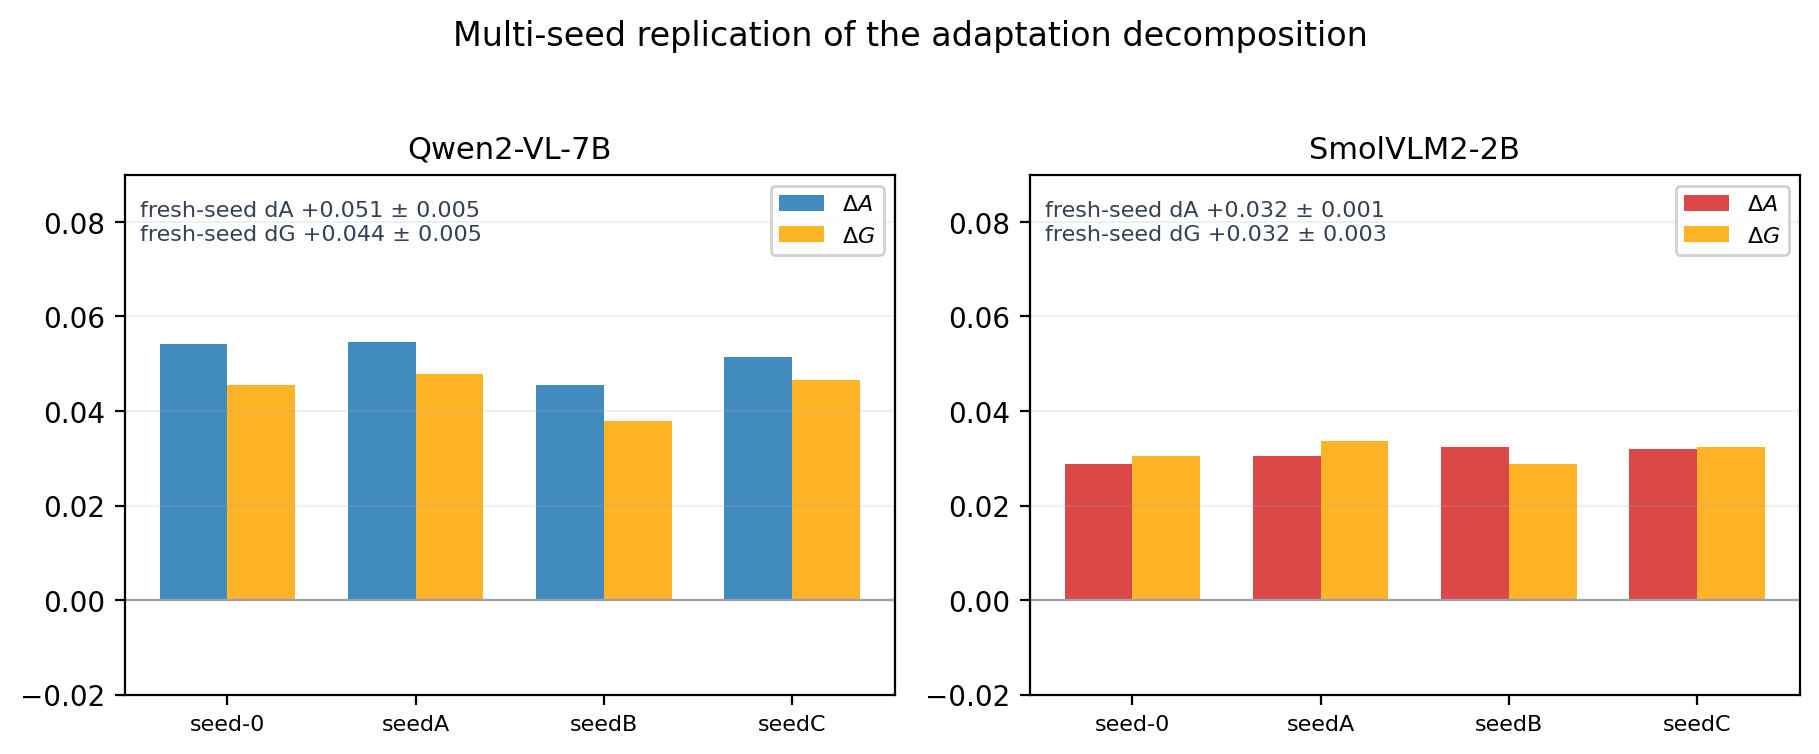
\includegraphics[width=\columnwidth]{fig/fig2_multiseed.png}
\caption{Multi-seed replication: per-seed \dA{} and \dG{} for both
confirmatory families, with fresh-seed mean $\pm$ SD annotations.}
\label{fig:multiseed}
\end{figure}

\paragraph{Contemporary-backbone extension (\qwennew{}, post-confirmatory).}
\Cref{tab:headline} includes the \qwennew{} row: \dA{} $+0.0323$, \dG{}
$+0.0355$, and hflip\_flip transformed accuracy $+0.0449$ (0.6571
$\rightarrow$ 0.7020). This extension is explicitly exploratory: it
computed only \dA{}, \dG{}, and $A_{\text{transform}}$; $C_{\text{pair}}$
was not computed for it, and no response-law-compliance claim is made.
It is labeled post-confirmatory external validation, not preregistered
confirmatory evidence.

\begin{figure}[t]
\centering
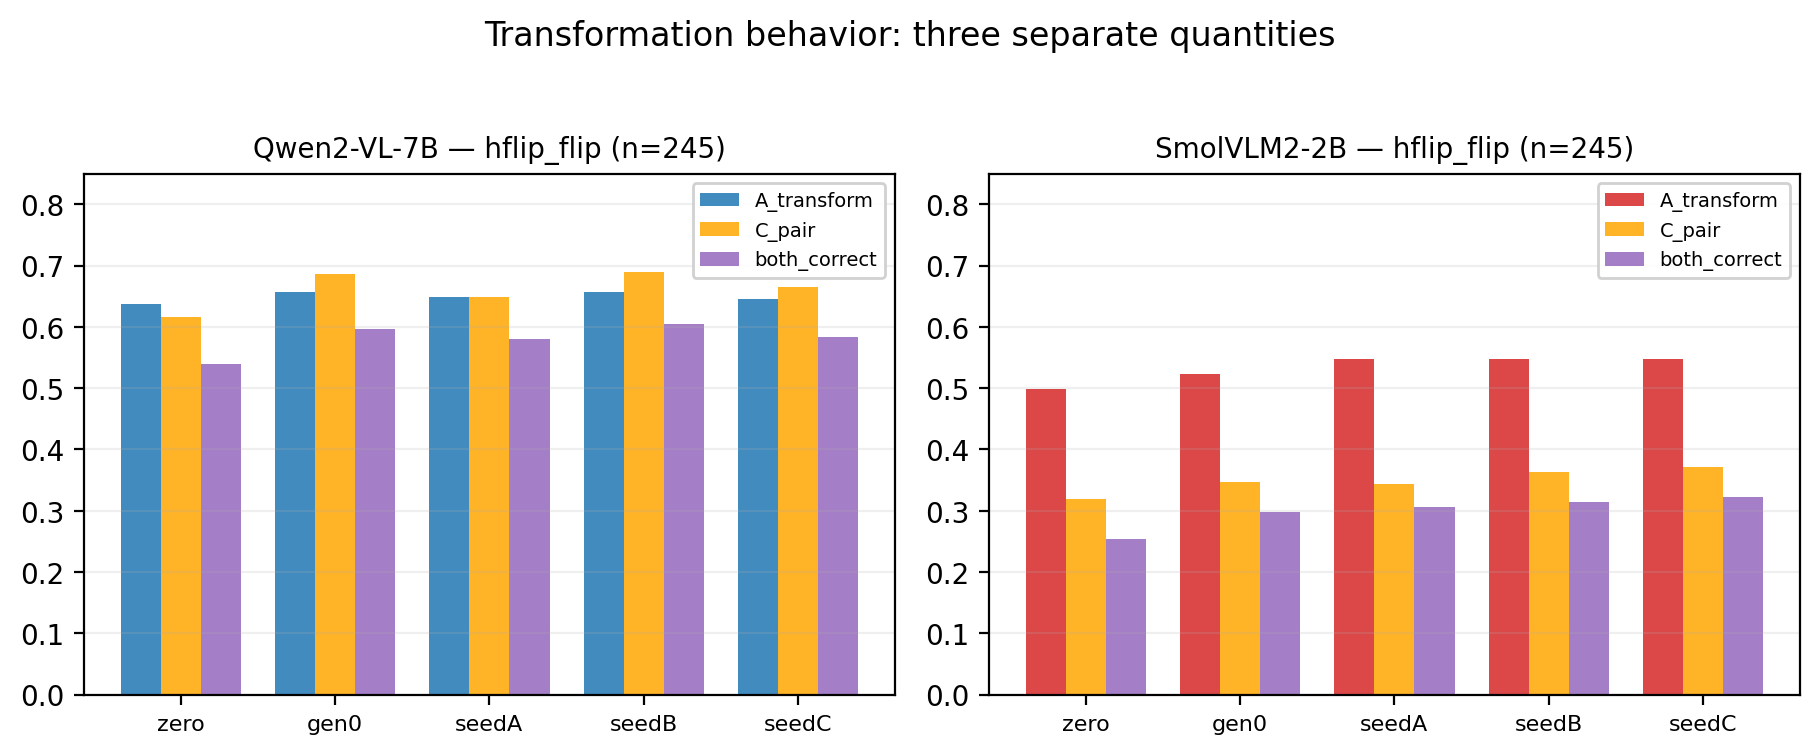
\includegraphics[width=\columnwidth]{fig/fig3_transform.png}
\caption{Transformation behavior: $A_{\text{transform}}$, $C_{\text{pair}}$,
and both\_correct per checkpoint, hflip\_flip ($n=245$), both families.}
\label{fig:transform}
\end{figure}

\paragraph{Claim-level summary (all audited).}
\begin{itemize}[leftmargin=*]
  \item \dA{} $> 0$ for all fresh seeds, both confirmatory backbones: PASS.
  \item \dG{} $> 0$ for all fresh seeds, both confirmatory backbones: PASS.
  \item Fresh-seed $C_{\text{pair}}$ within 0.05 of legacy General
        (7B and 2B): PASS.
  \item All fresh 2B hflip\_flip $C_{\text{pair}}$ $>$ 2B zero-shot: PASS.
  \item \qwennew{} supports only the stated \dA{}/\dG{}/
        $A_{\text{transform}}$ quantities: PASS.
\end{itemize}
